%        File: task-oriented_parser_evaluation.tex
%     Created: 周五 三月 02 04:00 下午 2012 W EST
% Last Change: 周五 三月 02 04:00 下午 2012 W EST
%
\documentclass[a4paper]{article}
%\usepackage{natbib}
%\usepackage{biblatex}
\usepackage{hyperref}
\usepackage{longtable}
%\usepackage[style=authoryear,natbib=true]{biblatex}
%\bibliography{D:/Research/bib/Parsing}
\usepackage{graphicx}
%\usepackage{gb4e}
\usepackage{lingmacros}
\usepackage{tikz}
\usepackage{tikz-qtree}
\title{Lexicalized Tree Adjoining Grammar Extraction For KBGEN}
\author{Wei Qiu \and Jiri Marsik}
%\date{}
\begin{document}
\maketitle
\begin{abstract}
\end{abstract}
\section{Introduction}


\section{Semantic Annotation}
\label{sec:sem-annot}

Extracting the elementary trees and aligning them to the triples
without any prior knowledge about the link between parts of the
sentences and the triples would have been very difficult. Therefore,
the first step of developing our system was to manually align sets of
triples to words from the sentences.

In order to shed light on the kind of alignment we were looking for, I
will list the properties we would like the alignment to have:

\begin{itemize}
\item Every word is aligned to some set of triples, i.e. every word is
  ``semantically motivated''. We would like our system to be able to
  generate the kind of sentences we had at the start. However, our
  surface realizer, GenI, never produces superfluous output (every
  word of the output is part of an elementary tree which was induced
  by some set of triples in the input).
\item Every triple is aligned to some set of words in the sentence.
  This is a reasonable requirement since the training sentences we
  have should be complete expressions of their semantic models.
  Furthermore, we would like to be able to generate at least the
  training data we have and GenI only considers generation successful
  if every semantic formula is realized via some elementary trees,
  which means there should not be any orphan triples.
\item The relation between the sets of words and sets of triples
  should be an alignment. By this, we mean to say that for every two
  different pairs of aligned sets of words and triples, the sets of
  words and the sets of triples should both be disjoint (in short, a
  word should not be aligned to two different sets of triples and a
  triple should not be aligned to two different sets of words).
\item The alignment we want to create should be the finest such
  alignment, meaning that any alignment which is a refinement of our
  alignment must lack one of the above properties. This is a natural
  requirement if we were doing things manually, since any rougher
  alignment can be easily arrived at by merging aligned groups.
  Furthermore, finer alignments will let us arrive at smaller
  elementary trees which generalize better, though they might
  overgenerate (which is a problem we were not afraid of, since we
  were afraid whether we will even be able to generate something).
\end{itemize}

For further discussion, we will label the sets of words that end up
aligned to some sets of triples \emph{groups}. Before we proceed with
a more linguistic description of the annotation guidelines, there is
one more technicality we would like to bring to light.

\subsection{Contiguous groups}

In our first rounds of annotation, we were working with an overly
strict constraint. Due to some confusion about how the realizer will
work and which realizer we will actually use, we restricted ourselves
to contiguous group only (groups whose all words form a contiguous
substring of the sentence). Under this constraint, we had trouble
accounting for several phenomena, the first one being conjunction.
Coordination was particularly tricky and required special treatment
even without the contiguity constraint (see Section \ref{ssec:coord}
for more details). However, other phrase structures such as ``... X
\textbf{, which also requires} Y \textbf{,} ...'' (mind the second
comma) with the semantics (X, requires, Y) or ``\textbf{the function
of} X \textbf{is} Y'' with semantics (X, has-function, Y).

After a while, we realized that the groups that we were manually
forming would correspond exactly to the final elementary trees (it was
the only alignment between semantics and syntax we had, after all).
Therefore, the sets of words in a group would not have to be
contiguous at all (the yield of an elementary tree may have
substitution or foot nodes surrounded by (co-)anchors).

\subsection{Annotation guidelines}

The realization that the groups of the alignment will correspond to
elementary trees restricts the space of possible alignments
significantly. These restrictions came both from the surface
realization of the sentence, where we imagined an idealized parse tree
and made sure that the groups would correspond to sensible and
composable elementary trees in that parse tree. On the semantic side,
we also needed the semantic links from the set of triples assigned by
the alignment to line up with the syntactic links in the elementary
tree (the substitution and adjunction sites).

Here are the guidelines for several common situations:

\begin{itemize}
\item NPs are aligned to their entity declarations.
\item For simple intransitive or transitive verbs, the event entity
  declaration and the triples which specify the agent (and the
  patient or whatever role the object takes) are aligned to the verb.
\item In an $n$-nary conjunction, all of the $n-1$ interposed
  conjunctions (comma, \emph{and}) are aligned to specialized
  \textbf{coordinates} relations which group all the coordinated
  entities into a single artificial entity.
\item For prepositions, we align the preposition (e.g. ``X \textbf{of}
  Y'') to a single triple which links some two entities (X and Y). In
  the resulting grammar, the preposition will correspond to an
  auxiliary tree where one the two semantic links will correspond to a
  substitution site and the other to the adjunction site.
\end{itemize}

And here is our guideline for a more involved but quite common
scenario:

\begin{itemize}
\item ``\textbf{The function of} X[NP] \textbf{is to provide energy
  for} Y[NP] \textbf{to} Z[VP].''

  Everything in bold in the sentence above will form a single group.
  This will be aligned to the following triples: (X, has-function, Z),
  (Z, raw-material, X) and (Z, agent, Y).
\end{itemize}

In the last example, you can see that I use the same meta-variables
for parts of the input syntax and the semantic entities. I assume
there is a natural assignment of the entities of the semantic
representation to certain constituents in the phrase structure. This
assumption is based on the fact that some groups (elementary trees)
are aligned to entity declarations and the idea that these entities
could be propagated up the tree according to headedness. It was this
idea that gave us hope that it should be possible to provide semantic
indices for the generated elementary trees automatically.

\subsection{Problems}



\section{Preprocessing}

There was a long way before we could start work on the problem itself
and we had to write a few auxiliary programs along the way. This
section describes the major steps and the tools we used there.

\subsection{Parsing and headedness}

Our plan is to extract the elementary trees for a TAG from a treebank.
Since our corpus lacks phrase structure information, we ran an
off-the-shelf parser on it. The parser that we used for this task is
the Stanford parser.

At the outset, we had plans to use both the phrase structure and
dependency parses that the Stanford parser could produce. Previous
research has shown that having a dependency parse facilitates the task
of determining headedness, which is usually a subtask of elementary
tree extraction.

Finally, we have found a simpler way of getting the head information
directly in the phrase structure parse trees through a command line
switch in the Stanford parser.


Furthermore, the Stanford parser offers two pre-trained models for
parsing English, an unlexicalized one and a lexicalized one. We have
done the parsing using both of them and try to review their
performance. Their outputs were significantly different and both
performed their own idiosyncratic errors. We judged which of these
errors would likely be more harmful to the following grammar
extraction process and decided to stick with the output of the
unlexicalized parser (though the result of the unlexicalized parsing
almost as just as bad as that of the lexicalized one).

\subsection{Aggregating coordinations}
\label{ssec:coord}

When we started working on the manual alignment with our self-enforced
constraint to produce only contiguous groups (see section
\ref{sec:sem-annot}), one of the difficulties we faced was
coordination. Consider the following example:

\begin{verbatim}
Electrogenic pumps, which consist of a hydrophobic amino acid,
a polar amino acid and a monomer, create  membrane potential.

(KBGEN-INPUT 
    :TRIPLES (
            (|Electrogenic-Pump21300| |has-part| |Monomer21323|)
            (|Electrogenic-Pump21300| |has-part| |Polar-Amino-Acid21291|)
            (|Electrogenic-Pump21300| |has-part| |Hydrophobic-Amino-Acid21290|)
            (|Create21297| |agent| |Electrogenic-Pump21300|)
            (|Create21297| |result| |Membrane-Potential21299|))
    :INSTANCE-TYPES (
            (|Monomer21323| |instance-of| |Monomer|)
            (|Polar-Amino-Acid21291| |instance-of| |Polar-Amino-Acid|)
            (|Hydrophobic-Amino-Acid21290| |instance-of| |Hydrophobic-Amino-Acid|)
            (|Electrogenic-Pump21300| |instance-of| |Electrogenic-Pump|)
            (|Create21297| |instance-of| |Create|)
            (|Membrane-Potential21299| |instance-of| |Membrane-Potential|)))
\end{verbatim}

To what group should the comma and the conjunction \emph{and} belong,
i.e. what semantics correspond to them and only to them? The
\textbf{has-part} relations belong to the verb \emph{consists}, the
instance declarations belong to the NPs. Yet we need to assign the
coordination constructions to some semantics, otherwise we will not be
able to generate them. To resolve this issue, we have developed a tool
to reify the coordination structures within the triples themselves.

In our first approach, our program would look for every instance where
one entity was in the same relation with multiple entities, such as
above, and converted the triples to the following:

\begin{verbatim}
:TRIPLES (
        (|Coordination2085| |coordinates| |Monomer21323|)
        (|Coordination2085| |coordinates| |Polar-Amino-Acid21291|)
        (|Coordination2086| |coordinates| |Coordination2085|)
        (|Coordination2086| |coordinates| |Hydrophobic-Amino-Acid21290|)
        (|Electrogenic-Pump21300| |has-part| |Coordination2086|)
        (|Create21297| |agent| |Electrogenic-Pump21300|)
        (|Create21297| |result| |Membrane-Potential21299|))
\end{verbatim}

What we did is that we built a very specific kind of binary tree which
covers the coordinated entities (the generated tree is specific in
that it always leans to the right, so it looks more like a linked
list). Here, one \textbf{Coordination} entity,
\textbf{Coordination2085}, subsumes the \textbf{Monomer21323} and the
\textbf{Polar-Amino-Acid21291}. This coordination corresponds to the
conjunction \emph{and}. The second coordination connects another
entity, the \textbf{Hydrophobic-Amino-Acid21290}, to the previously
formed \textbf{Coordination2085}. The resulting
\textbf{Coordination2086} can then serve as the singular object to the
verb \emph{consists}. Now, all of the NP coordinating constructs
(commas and \emph{and}) are easily accounted for. They form singleton
groups that are aligned to a pair of \textbf{coordinates} relations.

Once we made the switch from contiguous groups, we revised our
approach to coordination. Instead of making this hierarchy of
coordination constructs, we just create a single \textbf{Coordination}
entity which encapsulates all of the coordinated entities directly.
Obviously, this would not have been possible for coordinations of more
than 2 constituents using only contiguous groups, since we would not
to place two non-adjacent conjunction markers into one group.

The upsides of this new approach are that it reduces the complexity of
the newly added triples and that it does not overgenerate like the
last approach, which would end up extracting two elementary trees for
conjunction (one for comma and one for \emph{and}), but would not be
able to distinguish between them and use them properly. The only
downside of the new approach is that it needs to learn different
elementary trees for each different arity of conjunction present in
the corpus. However, since the number of coordinated constituents is
always between 2 and 4 in our corpus, this is a non-issue.

Here is the above example, now rendered using the new coordination
aggregation rules:

\begin{verbatim}
    :TRIPLES (
            (|Electrogenic-Pump21300| |has-part| |Coordination2015|)
            (|Coordination2015| |coordinates| |Monomer21323|)
            (|Coordination2015| |coordinates| |Polar-Amino-Acid21291|)
            (|Coordination2015| |coordinates| |Hydrophobic-Amino-Acid21290|)
            (|Create21297| |agent| |Electrogenic-Pump21300|)
            (|Create21297| |result| |Membrane-Potential21299|))
\end{verbatim}

The code for performing the former aggregation method is still present
in the aggregation program, but is no longer used (see function
\texttt{coordinate-objects-list}). Switching to the new method was
just a matter of writing a new function,
\texttt{coordinate-objects-flat}, and calling that one instead of the
former.

\subsection{Normalizing}

Once we had the manually aligned data with the aggregated
coordinations and parsed sentences, we thought ourselves ready to
extract the elementary trees. However, the trees produced by the
Stanford producer do not look very much like derived trees produced by
a TAG.

Xia and Palmer were facing a similar problem (\emph{From Treebanks to
Tree Adjoining Grammars}). We considered applying their approach.
However, their approach is not as simple as it seems on paper.
Consider the following parse tree we got from 

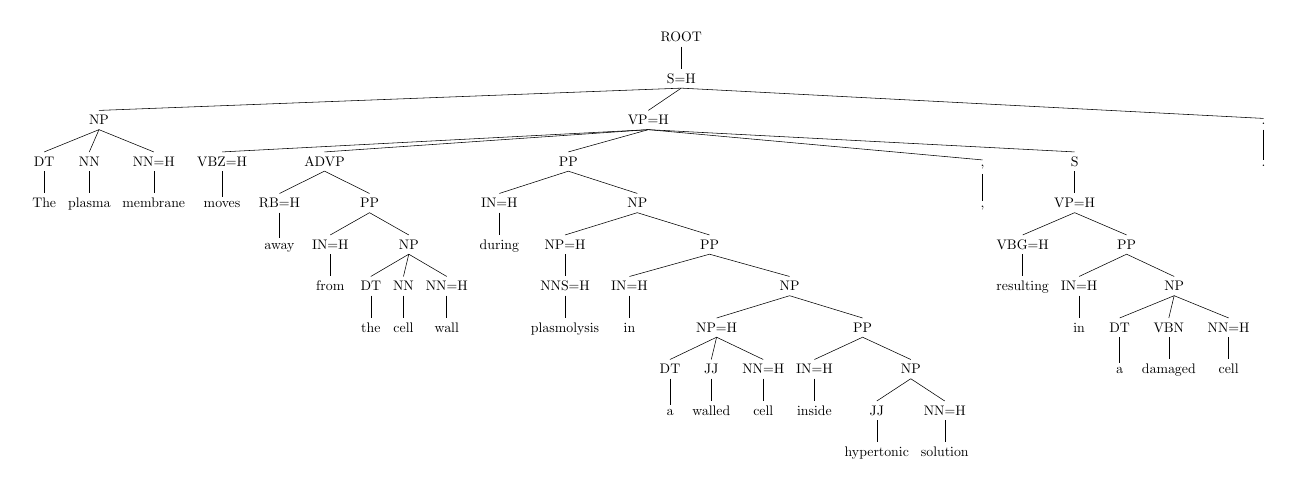
\begin{tikzpicture}[scale=0.5]
\Tree
[.ROOT
  [.S=H
    [.NP [.DT The ] [.NN plasma ] [.NN=H membrane ] ]
    [.VP=H [.VBZ=H moves ]
      [.ADVP [.RB=H away ]
        [.PP [.IN=H from ]
          [.NP [.DT the ] [.NN cell ] [.NN=H wall ] ] ] ]
      [.PP [.IN=H during ]
        [.NP
          [.NP=H [.NNS=H plasmolysis ] ]
          [.PP [.IN=H in ]
            [.NP
              [.NP=H [.DT a ] [.JJ walled ] [.NN=H cell ] ]
              [.PP [.IN=H inside ]
                [.NP [.JJ hypertonic ] [.NN=H solution ] ] ] ] ] ] ]
      [., , ]
      [.S
        [.VP=H [.VBG=H resulting ]
          [.PP [.IN=H in ]
            [.NP [.DT a ] [.VBN damaged ] [.NN=H cell ] ] ] ] ] ]
    [.. . ] ] ]
\end{tikzpicture}

The PP \emph{``during...''} and the S \emph{``resulting...''} with its
preceding comma both modify their parent, the VP of our sentence. We
can imagine that in our implementation of the algorithm, these would
be identified as modifiers and they would be put on different levels
from the argument ADVP, like so.

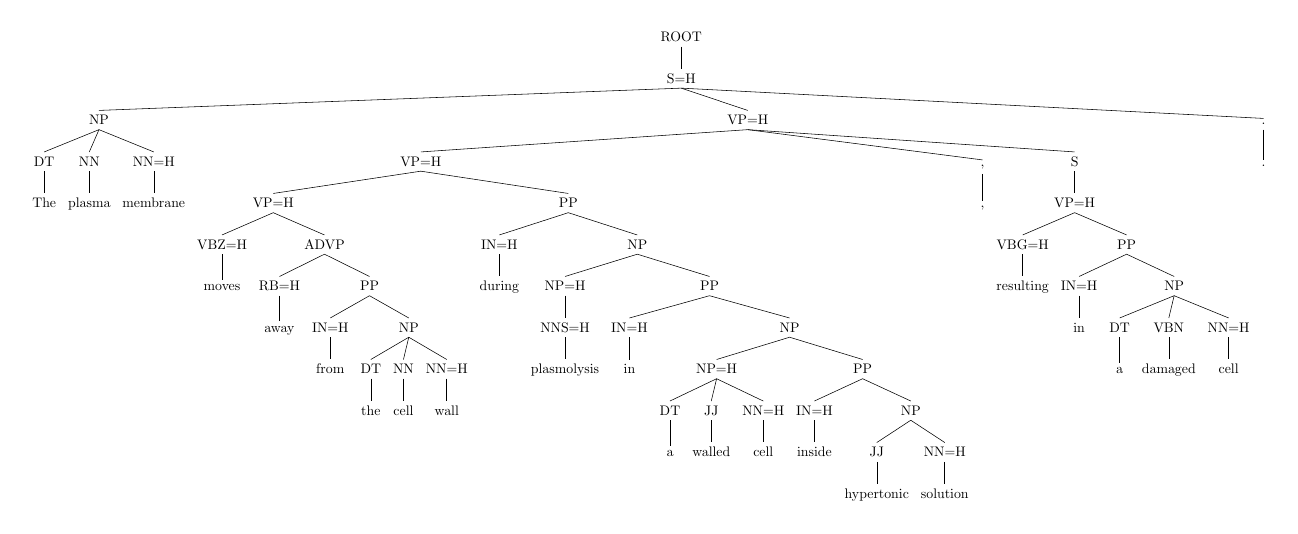
\begin{tikzpicture}[scale=0.5]
\Tree
[.ROOT
  [.S=H
    [.NP [.DT The ] [.NN plasma ] [.NN=H membrane ] ]
    [.VP=H
      [.VP=H
        [.VP=H [.VBZ=H moves ]
          [.ADVP [.RB=H away ]
            [.PP [.IN=H from ]
              [.NP [.DT the ] [.NN cell ] [.NN=H wall ] ] ] ] ]
        [.PP [.IN=H during ]
          [.NP
            [.NP=H [.NNS=H plasmolysis ] ]
            [.PP [.IN=H in ]
              [.NP
                [.NP=H [.DT a ] [.JJ walled ] [.NN=H cell ] ]
                [.PP [.IN=H inside ]
                  [.NP [.JJ hypertonic ] [.NN=H solution ] ] ] ] ] ] ] ]
      [., , ]
      [.S
        [.VP=H [.VBG=H resulting ]
          [.PP [.IN=H in ]
            [.NP [.DT a ] [.VBN damaged ] [.NN=H cell ] ] ] ] ] ]
    [.. . ] ] ]
\end{tikzpicture}

So far so good, nice and consistent. However, then we look at the NPs
and we see that the adjectives are sisters to the nouns that they
modify.

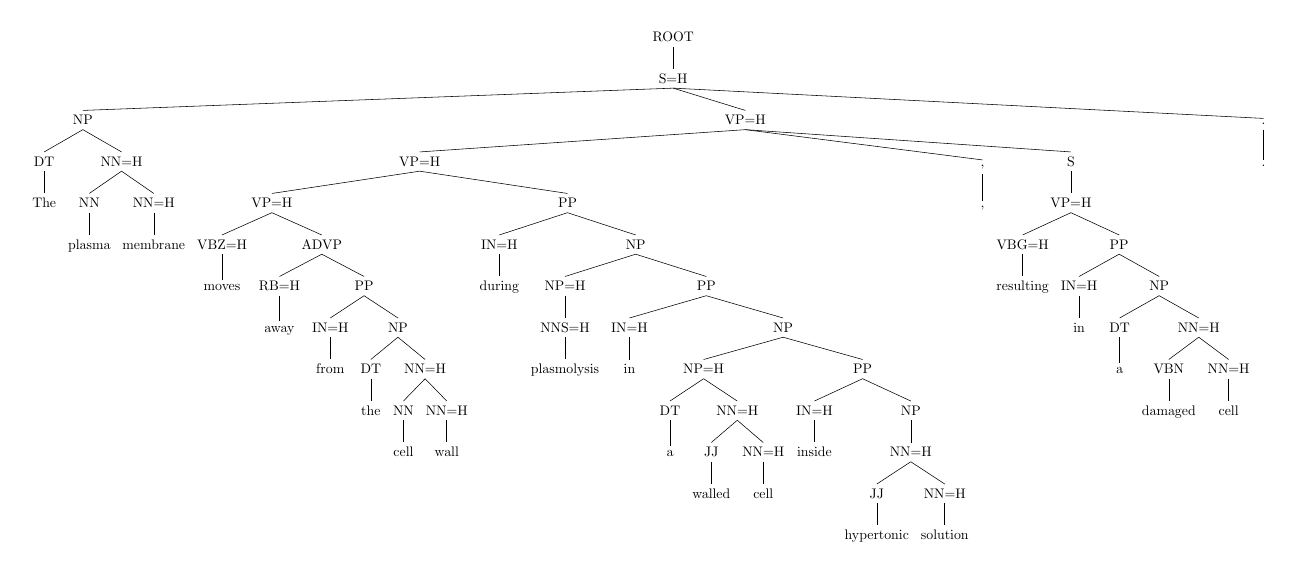
\begin{tikzpicture}[scale=0.5]
\Tree
[.ROOT
  [.S=H
    [.NP [.DT The ] [.NN=H [.NN plasma ] [.NN=H membrane ] ] ]
    [.VP=H
      [.VP=H
        [.VP=H [.VBZ=H moves ]
          [.ADVP [.RB=H away ]
            [.PP [.IN=H from ]
              [.NP [.DT the ] [.NN=H [.NN cell ] [.NN=H wall ] ] ] ] ] ]
        [.PP [.IN=H during ]
          [.NP
            [.NP=H [.NNS=H plasmolysis ] ]
            [.PP [.IN=H in ]
              [.NP
                [.NP=H [.DT a ] [.NN=H [.JJ walled ] [.NN=H cell ] ] ]
                [.PP [.IN=H inside ]
                  [.NP [.NN=H [.JJ hypertonic ] [.NN=H solution ] ] ] ] ] ] ] ] ]
      [., , ]
      [.S
        [.VP=H [.VBG=H resulting ]
          [.PP [.IN=H in ]
            [.NP [.DT a ] [.NN=H [.VBN damaged ] [.NN=H cell ] ] ] ] ] ] ]
    [.. . ] ] ]
\end{tikzpicture}

This asymmetry in the parser output made the approach of implementing
a procedure like theirs that would handle all of the flattening
phenomena in one unified manner seem not so viable. Instead, we chose
to implement a simple rule-based logic program to solve the flattening
we have discovered in our data.

We implemented two deflattening rules. One rule handled the general
case demonstrated on the PP and SBAR modifying the VP. This rule uses
a simple heuristic to determine whether a child of a node with more
than two children is a modifier or not. We refined this heuristic by
querying the output of the program and modifying the rules to account
for unforeseen circumstances. The final rule for detecting
modifiers/adjuncts follows.

A is an adjunct if one of the following is true:

\begin{itemize}
\item A is a PP
\item A is an S which does not have the form [S [VP=H [TO=H to] ...]]
\item A is a comma (we treat commas as adjuncts, so that, along with
  the ``real'' adjunct, they will form a two-level auxiliary tree)
\item A is an SBAR of the form [SBAR [WHNP=H [WDT=H which]] ...]
  (appositive relative clauses)
\end{itemize}

The second rule we have implemented is specialized for NPs. We look at
every noun in a final position (the last child of an NP or one that is
followed by a comma or a conjunction, since the Stanford parser
sometimes even flattens entire conjunctions of nouns, see below). For
every such noun, we look at its left sister and if it is a permissible
modifier (NN, NNP, JJ, VBN or ADJP). If so, we can mark the modifier
as an adjunct and put it together with the noun under a new noun tag.

This tree then...

\Tree
[.NP [.NN activation ] [.NN energy ]
     [.CC and ]
     [.NN water ] [.NNS=H molecules ] ]

...becomes this...

\Tree
[.NP [.NN [.NN activation ] [.NN energy ] ]
     [.CC and ]
     [.NNS=H [.NN water ] [.NNS=H molecules ] ] ]

After applying these two rules, we have examined all the possible
problem sites. That is, the nodes which had more than two children
after the deflattening (possible false negatives of our deflatter) and
all the adjunctions performed by our deflatter (possible false
positives). Upon their inspection, we have not found much room for
improvement and declared our algorithm finished.

The downside of this approach is that the further refining of our
heuristic predicates would get much harder as the size and variety of
our corpus grew larger. The upside is that it handles the language
found in our corpus very well and it has a short and (hopefully)
transparent implementation. For a discussion of some of the uncommon
implementation techniques we used, see the post at the following link.

\texttt{http://jirka.marsik.me/2012/12/19/the-working-hipster-s-clojure/}

\section{TAG extraction}
\section{Semantic roles alignment}
\section{Implementation and result}
data format
\section{Conclusion \& Future work}
\subsection{Future work}
\begin{itemize}
    \item workaround with parsing errors.
    \item more robust extraction algorithms
    \item more robust alignment algorithms
\end{itemize}
\end{document}
